\documentclass[12pt,preprint]{elsarticle}
\usepackage{amsmath, amssymb, amsthm}
\usepackage{rotating}
\usepackage{subfigure}

\usepackage{algorithm}
\usepackage{algorithmic}

\journal{Decision Support Systems}

\usepackage{a4wide}
\usepackage{amsmath, amsfonts, amssymb}
\usepackage{pb-diagram}
\usepackage{graphicx}
\usepackage{subfigure}
\usepackage{tikz}

\usepackage[dvipsnames, svgnames, x11names]{xcolor}
\usepackage{color}

\newcommand{\blambda}{\boldsymbol{\lambda}}
\newcommand{\bz}{\mathbf{z}}
\newcommand{\bx}{\mathbf{x}}
\newcommand{\by}{\mathbf{y}}
\newcommand{\bw}{\mathbf{w}}
\newcommand{\bZ}{\mathbf{Z}}
\newcommand{\bA}{\mathbf{A}}
\newcommand{\btheta}{\boldsymbol{\theta}}
\newcommand{\bPsi}{\boldsymbol{\Psi}}
\newcommand{\bpsi}{\boldsymbol{\psi}}
\newcommand{\bchi}{\boldsymbol{\chi}}
\newcommand{\bzeta}{\boldsymbol{\zeta}}
\newcommand{\T}{^{\mathsf{T}}}
\newtheorem{Theorem}{Theorem}
\newtheorem{Ex}{Example}
\newtheorem{Def}{Definition}

\renewcommand{\baselinestretch}{1.5}

\begin{document}

%\begin{frontmatter}
\title{Ordinal Classification Using Partially Ordered Feature Sets}
 

\author[mipt]{I.\,D.~Papay}
\ead{papayid1503@gmail.com}

\author[mipt,ccas]{V.\,V.~Strijov}
\ead{strijov@ccas.ru}
\cortext[cor1]{Corresponding author}


\begin{abstract}
This paper presents a method to solve an ordinal classification problem where the objects are described with a set of partially ordered features.
To construct an ordinal classification model we aggregate partial orders of features by weighting the incidence matrices of partial order graphs. To describe set of possible solutions we use partial order cones corresponding to the incidence matrices and find a solution of the classification problem as the projection of a vector of response variables to a superposition of the cones. We propose a method of optimum parameter estimation for the ordinal classification model. The method is applied to the Football Player List categorization problem.
\end{abstract}

\begin{keyword}
ordinal classification, alternatives ranking, preference learning, partial order, monotonic constraints
\end{keyword}

\maketitle

\section{Introduction}
We consider an ordinal classification problem using partially ordered feature sets. This problem generalizes the well-known ordinal classification problem with monotonic constraints~\cite{Kotlowski2013, Corrente2013, Ali2020}. The objective is to construct a monotonic function, further calling a classification model, mapping an object set to a class label set such that the class label set is strictly totally ordered. The requirement of the classification model monotonicity is a form of prior knowledge of a relation between a response and predictor variables~\cite{raey, Jorge2024, Eduardo2022}. The motivation for this type of problem statement arises in areas of support decision theory~\cite{Enrique2023,Ameed2022,Yossi2022}, information retrieval~\cite{Schafer2007,Trotman2005,Spirin2011} and preference learning~\cite{Fuernkranz2011, Bofei2024}.

The task is set as follows. There are a number of experts ranking some partially ordered set of objects. Our goal is to teach the model to predict the rank~\cite{Nadia2020} of an individual object for any other expert~\cite{Elena2023}. At the same time, all that is known about an object is a finite-dimensional vector of its features. 

In this paper we consider a general case of classification model monotonicity requirement: the set of values for each feature is a partially ordered set, that is, a partial order relation is defined over the feature values set~\cite{Cheng2010}. The goal is to construct a classification model satisfying monotonicity of relation between partially ordered features and a response variable. To construct a classification model defined over the Cartesian product of the partially ordered sets, we use incidence matrices of the graphs corresponding to the partial orders. We introduce a partial order cone corresponding to the incidence matrix~\cite{Kuznetsov2014, Dehnokhalaji2011256}. We regard a superposition of the partial order cones as the set of possible solutions of the ordinal classification problem. In the paper we prove that the constructed cone superposition describes a broad class of monotonic transformations.

As a solution of the ordinal classification problem we find a point in the superposition of the cones, maximizing its correlation with the expert-given target vector. We propose a method of parametrization of the cone superposition to find optimal parameters of the classification model. Using this parametrization, the method of parameter estimation consists of the two independent stages. In the first stage we construct a matrix of pairwise dominance of the objects. This type of matrices is used in alternatives ranking problems~\cite{Kaci2011,Busa-Fekete2013}. In the paper~\cite{Cohen1999} the authors solve a problem of the linear order construction using the pairwise dominance matrix. In the second stage we solve an ordinal classification problem wherein using the columns of the dominance matrix as the new predictor variables.

In this paper we investigate properties of the partial order cone generators. We show that the generator vectors are equal to the columns of the incidence matrix corresponding to the partial order. This novel fact proves that the proposed method of ordinal classification finds an optimal function in a sufficiently broad class of monotonic transformations.

As methods competing with the proposed method, that solves our problem, we assume decision oblique trees and isotonic regression.

Decision tree can be explained a series of nested if-then-else statements. Each  non-leaf  node  has  a  predicate  associated, testing an  attribute of data.  Terminal node  denotes class, or category. To classify a data ,we have to traverse down the tree by starting  from root  node ,testing predicates( test attribute) and taking branches labelled with corresponding value.

Isotonic regression is a technique used to fit a non-decreasing function to a set of data points.
We can think of isotonic regression as a generalization of linear regression where the function is constrained to be non-decreasing.

The proposed method is compared with oblique decision tree~\cite{Wilhelm2021} and isotonic regression~\cite{SALMON2017} on synthetic and real data. As a real data we consider a problem of the Football Player List categorization, also described in. The goal is to rank FIFA players by their world reputation ranks basing on their characteristics. The following categories are considered: least popular, rarely heard, normally heard, popular, extremely popular. This categorization is monotonic. The partially ordered features (e.g., mobility, strength) are given by the experts. The proposed method shows better results in comparison with the alternative approaches.

\begin{table}[!htbp]
\label{tab:intro_comparative}
\caption{Comparative analysis of basic solution to my problem.}
\begin{tabular}{p{5cm}|p{5cm}|p{5cm}}
	Solution & Strengths & Weakness \\
	\hline
	Partial Orders & 
	no contradictions in the partial order &
	vulnerable to noise \\
    \hline
	Isotonic regression & 
	working fast &
	inaccurately predictions \\
    \hline
	Oblique decision trees & 
	learns non-linearity dependence &
	vulnerable to retraining \\
    \hline
	Stochastic Partial Orders & 
	no vulnerability to noise &
	demand higher dimension of features \\
\end{tabular} 
\end{table}

\section{Ordinal classification with monotonicity constraints}
\paragraph{Partially ordered feature set}
Let~$\mathfrak{D}$ be a sample consisting of the pairs
\[
\mathfrak{D}=\{(\bx_i,y_i)\}_{i=1}^m,
\label{eq:Sample}
\]
where~$\bx_i=[x_{i1},...,x_{ij},...,x_{in}]\T$~is an object to be classified, $y_i$~is a class label. An object~$\bx_i$ is an $n$-dimensional vector, each component of which belongs to the corresponding partially ordered set~$X_j$. In other words, an element~$j$ of the vector~$\bx_i$ (which is also reffered to as value of the feature~$j$ for the object~$\bx_i$) belongs to the set~$X_j$ with the given partial order relation~$\succeq$ with the following properties:
\begin{itemize}
\item reflexivity, $\forall a\in X$ $(a\succeq a)$,
\item antisymmetry, $\forall a,b\in X$, $(a\succeq b)\wedge(b\succeq a)\Rightarrow (a= c)$,
\item transitivity, $\forall a,b,c\in X$ $(a\succeq b)\wedge(b\succeq c)\Rightarrow (a\succeq c)$.
\end{itemize}
Thereby the object set~$X$ is a Cartesian product of the partially ordered sets~$X_1,...,X_n$,
\[
X=X_1\times X_2\times \dots \times X_n,
\]
the sets~$X_1,...,X_n$ are the feature values sets.

Every partial order~$\succeq$, defined on a set~$X_j$, described with a binary function~$z_j(\bx_i,\bx_k)$ such that
\[
z_j(\bx_i,\bx_k)=
\begin{cases}
1,\quad\text{if}\quad x_{ij} \succeq x_{kj}, \\
0,\quad\text{if}\quad x_{ij}\nsucceq x_{kj},
\end{cases}
\]
where the function~$z_j(\cdot,\cdot)$ satisfies the conditions of reflexivity, antisymmetry and transitivity.

Let us define a partial order matrix~$\bZ_j$ for the sample~$\mathfrak{D}$ and every set~$X_j$ such that the matrix describes binary relation between each pair of the sample elements,
\[
\bZ_j(i,k) = z_j(\bx_i,\bx_k),
\]
where~$j$~ is a feature index, and~$i,k$~are the object indices.
Note that for the matrix~$\bZ_j$, as well as for the function~$z_j$, elements~$\bZ_j(i,k)$~and~$\bZ_j(k,i)$ do not depend on each other. For example, the objects~$i,k$ can be incomparable with each other for the feature~$j$. In this case for the matrix~$\bZ_j$ the following equalities hold:
\[
\bZ_j(i,k)=\bZ_j(k,i)=0.
\]
On the other hand, the objects~$i,k$ can be equal for the feature~$j$. In this case, the following equalities hold:
\[
\bZ_j(i,k)=\bZ_j(k,i)=1.
\]
\begin{Ex}
The partially ordered set~$X_j$ consists of four objects with the following binary relation,
\[
X_j=\{x_{1},x_{2},x_{3},x_{4}|\;x_{1}\succeq x_{2}, x_{2}\succeq x_{3}, x_{2}\succeq x_{4}\}.
\]
The partial order on the objects~$x_{1},x_{2},x_{3},x_{4}$ is described by a partial order graph,
\[
\begin{diagram}
\node{x_{1}} \arrow[2]{e}{}
\node[2]{x_{2}} \arrow[2]{}
\arrow{se,b}{}
\node[2]{x_{3}} \\
\node[4]{x_{4}}
\end{diagram}
\]
This graph corresponds to a matrix~$\bZ_j$:
\[
\bZ_j=
\begin{pmatrix}
1 & 1 & 1 & 1 \\
0 & 1 & 1 & 1 \\
0 & 0 & 1 & 0 \\
0 & 0 & 0 & 1 \\
\end{pmatrix}.
\]
\label{ex1}
\end{Ex}
The class label set
\begin{equation}
Y=\{l_1,l_2,...,l_K\},\quad y_i\in Y
\label{yValues}
\end{equation}
is a finite set with the specified strict linear order relation,~$l_1\prec l_2,...,\prec l_K$, where~$K$~is a number of the class labels. Similarly to the matrices~$\bZ_1,...,\bZ_n$, construct a partial order matrix~$\bZ_0$ corresponding to the vector of class labels~$\by=[y_1,...,y_m]\T$ of the sample~$\mathfrak{D}$:
\[
\bZ_0(i,k) =
\begin{cases}
1,\quad\text{if } y_i\succeq y_k, \\
0,\quad\text{otherwise}.
\end{cases}
\]
\paragraph{Partial order cone}
Introduce a polyhedral cone~$\mathcal{X}$, corresponding to the partially ordered set of feature values.
\begin{Def}
A polyhedral cone in~$\mathbb{R}^m$~is a set~$\mathcal{X}$ such that
\[
\mathcal{X}=\{\bchi\;|\;\bA\bchi\leq \mathbf{0},\;\bchi\in\mathbb{R}^m\},
\]
fore some matrix~$\bA$.
\end{Def}

By matrix $A$ in our article, from here on, we consider the matrix
\[
\bA_m=
\begin{pmatrix}
-1 & 1 & 0 & \dots & 0 & 0 \\
0 & -1 & 1 & \dots & 0 & 0 \\
\vdots & \vdots & \vdots & \ddots & \vdots & \vdots \\
0 & 0 & 0 & \dots & -1 & 1 \\
0 & 0 & 0 & \dots & 0 & -1 \\
\end{pmatrix},
\]

For each set~$X_j$ define a cone~$\mathcal{X}_j$ in a space~$\mathbb{R}^m_+$:
\begin{equation}
\mathcal{X}_j=\{\bchi_j\in\mathbb{R}^m_+|\quad x_{ij}\succeq x_{kj}\rightarrow \chi_{ij}\geq \chi_{kj}\quad \forall i,k=1,...,m\},
\label{ConeDef}
\end{equation}
where~$x_{ij}$~and~$x_{kj}$~are values of the feature~$j$ on the sample elements~$i$~and~$k$, respectively.
For the cone~$\mathcal{X}$ (index~$j$ is omitted for the reasons of convenience) the following theorem holds.
\begin{Theorem}
A vector~$\bchi$ belonging to the cone~$\mathcal{X}$ can be represented as the nonnegative combination of cone generators,
$$\bchi=\sum\limits_{k=1}^{m}\lambda_{k}\bzeta_{k}, \quad\lambda_{k}\geq 0,$$
where~$\bzeta_k$~is a generatrix of the cone~$\mathcal{X}$,
\[
\bzeta_{k}(i)=
\begin{cases}
1,\quad \text{if}\quad x_i\succeq x_k,\\
0,\quad\text{if}\quad x_i\nsucceq x_k,
\end{cases}
\]
and this decomposition is unique.

\begin{tikzpicture}[>=stealth]
\draw[thick, ->, black] (0,0) -- (12,0);
\draw[thick, ->, red] (0,0) -- (6,0);

\draw[thick, ->, black] (0,0) -- (0,12);

\draw[ultra thick, black] (0,0) -- (9,9);
\draw[ultra thick, ->, red] (0,0) -- (4.5,4.5);

\draw[thick, blue] (5.25,5.25) -- (8.25, 2.625) -- (8.25, 0);



\draw[dashed] (9,9) -- (11.25,0);

\node[below left] at (0,12) {\color{black}$\mathcal{X}_1$};
\node[below right] at (12,0) {\color{black}$\mathcal{X}_2$};
\node[above right] at (9,9) {\color{black}$\mathcal{X}$};
\node[above right] at (8.25, 2.625) {\color{black}$\mathcal{X}$};

\node[below right] at (5.85,0) {\color{red}$\bzeta_{2}$};
\node[above right] at (4.0,4.5) {\color{red}$\bzeta_{1}$};

\node[below right] at (8.45,1.3) {\color{blue}$\lambda_{2}$};
\node[above right] at (7.0,3.5) {\color{blue}$\lambda_{1}$};

\end{tikzpicture}


The figure illustrates vector~$\bchi$ decomposition on the generators~$\bzeta_1,\bzeta_2$ of the cone~$\mathcal{X}$. The vector~$\bchi\in \mathcal{X}$ is a nonnegative combination of the generators~$\bzeta_1=[1;1]$~and~$\bzeta_2=[1;0]$ with the coefficients~$\lambda_1,\lambda_2\geq 0$.

Theorem 1 establishes the following connection between the cone~$\mathcal{X}_j$ and the partial order matrix~$\bZ_j$: the generatrix~$\bzeta_{jk}$ of the cone~$\mathcal{X}_j$ is a column~$k$ of the matrix~$\bZ_j$.

\paragraph{Ordinal classification with monotonicity constraints}
In this section we formulate the problem of ordinal classification with monotonicity constraints; the constraints monotonicity means satisfying the given object binary relations.

As it was mentioned before~(\ref{yValues}), the set of class labels~$Y=\{l_1,l_2,...,l_K\}$~is a finite set with the specified strict linear order relation,~$l_1\prec l_2,...,\prec l_K$. The goal is to construct a monotonic function~$f:X\rightarrow Y$ minimizing a given loss function,
\begin{equation}
S(\mathfrak{D})=\sum\limits_{i=1}^m{s(f(\bx_i), y_i)}\rightarrow \min,
\label{ErrGen}
\end{equation}
where~$s(f(\bx_i), y_i)$ is a loss value of the function~$f$ on the object~$\bx_i$.
We construct a monotonic function~$f$ as the following superposition,
\begin{equation}
f(\bx)=\phi(u(\bx)),
\label{problOrdClass}
\end{equation}
where~$u:X\rightarrow \mathbb{R}$ is a \emph{utility function} mapping object set~$X$ to the real axis~$\mathbb{R}$, and $\phi:\mathbb{R}\rightarrow Y$ is a \emph{decision rule} dividing the real axis into the sets of correspondence to the class labels~$l_1,...,l_K$.

Using conic description of the partially ordered sets~(\ref{ConeDef}), find a solution of the problem~(\ref{problOrdClass}) as follows. Find a vector~$\hat{\by}\in \mathbb{R}^m$ that belongs to the superposition of the cones~$\mathcal{X}_1,...,\mathcal{X}_n$ and minimizes the loss function~(\ref{ErrGen}),
\[
S(\mathfrak{D})=\sum\limits_{i=1}^m{s(\phi(\hat{y}_i), y_i)}\rightarrow \min,\quad \hat{\by}\in \sum\limits_{i=1}^n\mathcal{X}_i,
\]
where~$\sum\limits_{i=1}^n\mathcal{X}_i$ denotes a Minkowski sum of the sets~$\mathcal{X}_1,...,\mathcal{X}_n$:
\[
\sum\limits_{i=1}^n\mathcal{X}_i=\{\bchi_1+...+\bchi_n\;|\;\bchi_1\in\mathcal{X}_1,...,\bchi_n\in\mathcal{X}_n\}.
\]
Note that though a Minkoswski sum of the cones~$\mathcal{X}_1,...,\mathcal{X}_n$ is a special case of a superposition of the sets~$\mathcal{X}_1,...,\mathcal{X}_n$, it still defines a sufficiently broad class of monotonic transformations. The concept of Minkowski sum generalizes \emph{linear model} idea in the case of ordered feature sets.

As long as target vector~$\hat{\by}$ must belong to the Minkowski sum of the cones,~$\hat{\by}\in \sum\limits_{i=1}^n\mathcal{X}_i$, from Theorem 1 it follows that the vector~$\hat{\by}$ decomposes in a linear combination of generators of the cones~$\mathcal{X}_1,...,\mathcal{X}_n$,
\[
\hat{\by}=\sum\limits_{j=1}^n\sum\limits_{k=1}^m\lambda_{jk}\bzeta_{jk},\quad \lambda_{jk}\in\mathbb{R}_+,
\]
where~$\bzeta_{jk}$~is a~$k$~-generatrix of the cone~$\mathcal{X}_j$. The vector~$\bzeta_{jk}$ is also a $k$~column of the partial order matrix~$\bZ_j$.
Therefore the utility function~$u$ from the formula~(\ref{problOrdClass}) for any object~$\bx\in X$ is as follows,
\begin{equation}
u(\bx) = \sum\limits_{j=1}^n w_j \sum\limits_{k=1}^m\lambda_{jk}z_j(\bx, \bx_k),
\label{utilityDecomp}
\end{equation}
where the parameters~$w_j$ are feature weights.

Note that the problem statement~(\ref{utilityDecomp}) is equivalent to a canonical problem of ordinal classification with monotonic constraints. The problem is to find a utility function~$u$ as a linear combination of monotonic functions~$u_1,...,u_n$:
\begin{equation}
u(\bx)=\sum\limits_{j=1}^n w_j u_j(x_j),
\label{problLinearMon}
\end{equation}
where every function~$u_j$ is monotonic due to its argument~$x\in X_j$,
\begin{equation}
x_2 \succeq x_1 \quad\rightarrow\quad u_j(x_2) \geq u_j(x_1).
\label{condMon}
\end{equation}

For the further considerations make some restrictions over a class of functions~$u(\bx)$.
Rewrite a formula~(\ref{utilityDecomp}) as follows,
\begin{equation}
u(\bx) = \sum\limits_{k=1}^m \lambda_{k} \sum\limits_{j=1}^n w_j z_j(\bx, \bx_k) = \sum\limits_{k=1}^m \lambda_{k} \Psi(\bx, \bx_k).
\label{utilityDecompDual}
\end{equation}
The model~(\ref{utilityDecompDual}) has equal parameter values~$\lambda_k$ for all the features~$j$. In this case the parameters~$\lambda_k$ are the object weights for the sample~$\mathfrak{D}$.
The function~$\Psi(\bx_i, \bx_k)$ describes partial order relation between the objects~$\bx_i$~and~$\bx_k$ and takes values in the unit interval~$[0;1]$,
\[
\Psi(\bx_i, \bx_k)\in[0,1].
\]
The function~$\Psi(\bx_i, \bx_k)$ can be interpreted as the pairwise dominance degree between the objects $\bx_i$~and~$\bx_k$,~$\bx_i\succeq\bx_k$.

\paragraph{Loss function minimization for the optimal parameters search}
To solve the problem of ordinal classification with monotonic constraints~(\ref{ErrGen}), let us to formulate a problem of finding the optimal parameters of the model~(\ref{utilityDecompDual}).
According to formula~(\ref{ErrGen}), the optimal parameters~$\hat{\bw},\hat{\blambda}$ minimize the loss function
\[
(\hat{\bw},\hat{\blambda})=\arg\min\limits_{\bw,\blambda}\left(S(\mathfrak{D}|\bw,\blambda)\right)=\arg\min\limits_{\bw,\blambda}\left(\sum\limits_{i=1}^m{s(f_{\bw,\blambda}(\bx_i), y_i)}\right),
\]
where~$s(f_{\bw,\blambda}(\bx_i), y_i)$~--- is the value of loss on an object~$\bx_i$, and a monotonic function
\begin{equation}
f_{\bw,\blambda}(\bx_i) = \phi\left(\sum\limits_{k=1}^m \lambda_{k} \Psi(\bx_i, \bx_k)\right)
\label{ordClassMdl}
\end{equation}
is defined by the expressions~(\ref{problOrdClass})~and~(\ref{utilityDecompDual}).
The explicit form of the loss function~$S$, of the decision rule~$\phi$ and of the binary relation function~$\Psi$ will be considered in the next section.
\section{Classification methods}
\subsection{Isothonic regression}


More formally suppose that one collects $n$ sample points $y_1,\dots, y_n$ and has weights $w_1, \dots, w_n$ associated with each data point.

When no a priori weights are given, we can set $w_i = 1$ for all $i \in \llbracket 1, n \rrbracket$.

Then, the isotonic regression problem can be formulated as follows:

\begin{align}
\min_{x \in \mathbb{R}^n}
\frac{1}{2}
& \sum_{i=1}^{n} w_i (x_i - y_i)^2 \\
\text{s.t.} & \quad x_1 \leq x_2 \leq \ldots \leq x_n \nonumber
\end{align}

The formulation of the isotonic regression problem given in (10) is a quadratic program (QP) with linear constraints.
Using a matrix notation, introducing the matrix
$$A = \begin{pmatrix} 1 & -1 &                       &                       &    \\
  & 1  & -1                    &                       &    \\
  &    & \ddots & \ddots &    \\
  &    &                       & 1                     & -1\end{pmatrix}
 =
\begin{pmatrix}
a_1^\top \\
\vdots   \\
a_{n-1}^\top
\end{pmatrix}
 \in \mathbb{R}^{n-1 \times n}\enspace,
$$
the isotonic regression problem can be formulated as follows:

\begin{align}
\min_{x \in \mathbb{R}^n}
\frac{1}{2}
& \sum_{i=1}^{n} w_i (x_i - y_i)^2 \\
\text{s.t.} & \quad Ax \leq 0 \nonumber
\end{align}




In what follows we will write $W=\diag(w_1,\dots,w_n)$, assuming that $w_i > 0$ for all $i \in \llbracket 1, n \rrbracket$, so $W^{-1}= \diag(1/w_1,\dots,1/w_n)$.
Hence, we can rewrite the isotonic regression problem as


\begin{align}
\min_{x \in \mathbb{R}^n}
\frac{1}{2}
& (x-y)^\top W (x-y) \\
\text{s.t.} & \quad Ax \leq 0 \enspace.
\end{align}

\begin{algorithm}[ht]
\caption{PAVA}\label{alg:cap}
\begin{algorithmic}
\Require $y \in\mathbb{R}^n, w \in \mathbb{R}^n_{+}$
\STATE $r \leftarrow y$
\STATE $W \leftarrow y$
\STATE $J = [\{1\},\dots, \{n\}]$ \COMMENT{lists of blocks}
\STATE $i=1$ (index of list start at 0 here)
\WHILE{$i<n$}
    \IF{$r_i < r_{i-1}$} \COMMENT{Find adjacent violators and merge groups}
        \State $r_i \leftarrow \frac{W_i r_i + W_{i-1} r_{i-1}}{W_i + W_{i-1}}$
        \State $W_i \leftarrow W_i + W_{i-1}$
        \State $J_i \leftarrow J_i \cup J_{i-1}$
        \State Remove $r_{i-1}$, $W_{i-1}$ and $J_{i-1}$ from the lists
        \IF{$i > 1$}
            \STATE{$i\leftarrow i-1$}
        \ENDIF
    \ELSE
        \STATE{$i  \leftarrow i + 1$}
    \ENDIF
\ENDWHILE
\FOR{$i=1$ to len($J$)}
    \STATE{$r_{J_i} \leftarrow \bar{y}_{J_i} \mathbf{1}_{J_i}$}
    \COMMENT{Set the block to the average value}
\ENDFOR
\RETURN{$r, J$}
\end{algorithmic}
\end{algorithm}

Hence, the isotonic regression problem can be formulated as a convex quadratic program with linear constraints.

The intuition behind the PAVA algorithm is to merge adjacent blocks of constant values in the primal vector, as the targeted solution is simply the average of the observe signal over each block.
Hence, the algorithm aims at creating the blocks of constant values in the primal vector. The dual variables can be inferred from the  solution from the previous lemma.

\subsection{Decision oblique trees}

\paragraph{Univariate and multivariate decision tree}
Multivariate  decision  trees  differ  from  univariate  decision trees in the way they  test the  attributes.   Univariate decision trees  test  single  attribute  at  internal  node.  Multivariate decision tree several attribute participate in single node split test.    The  limitation  to  one  attribute  reduces the  ability  of expressing concepts, due to its disability in three forms.  Splits could only be orthogonal to axes, subtrees may be replicated and fragmentation. 

Univariate test using feature $x_i$ can only split a space with a boundary that is orthogonal to the $x_i$ axis. This results in larger trees and poor generalization.  The  multivariate  decision  tree-constructing algorithm selects not the best attribute but the best linear  combination of the attributes: $\sum_{i=1}^f w_i x_i>0$. $w_i$ are the weights associated with each feature  $x_i$ and  $w_0$ is the threshold to be determined from the data. Multivariate decision trees  differ from  univariate trees  as the  symbolic  features  are  converted  into  numeric  features. And all splits are binary, final weighted sum is numeric.

We examine decision trees that test a linear combination of the attributes
at each internal node. More precisely, let an example take the form $X = x1; x2; \dots xd$; $C_j$
where $C_j$ is a class label and the $x_i$ are real-valued attributes. The test at each node will
then have the form:

\begin{align}
\sum_{i=1}^d a_i x_i + a_{d+1} > 0.
\end{align}

Here $a_1; \dots ; a_{d+1}$ are real-valued coefficients. Because these tests are equivalent to hyperplanes at an oblique orientation to the axes, we call this class of decision trees oblique
decision trees.

\begin{algorithm}[ht]
\caption{CART}\label{alg:cap}
\begin{algorithmic}
\COMMENT{To induce a split at node T of the decision tree:}
    \COMMENT{Normalize values for all d attributes.}
    \State $L = 0$
    \WHILE{TRUE}
        \STATE $L=L+1$
        \COMMENT{Let the current split $s_L$ be $u \leq c$, where $u=\sum_{i=1}^d a_i x_i$}
        \FOR{$i=1$ to $d$}
            \FOR{$\gamma=-0.25$ to $0.25$}
                \COMMENT{Search for the $\sigma$ that maximizes the goodness of the split $u-\sigma(a_i+\gamma) \leq c$}
            \ENDFOR
            \COMMENT{Let $\sigma^*,\gamma^*$ be the settings that result in highest goodness in these 3 searches}
            \STATE $a_i=a_i-\sigma^*$
            \STATE $c=c-\sigma^* \gamma^*$
        \ENDFOR
        \COMMENT{Perturb c to maximize the goodness of $s_L$, keeping $a_1, \dots, a_d$ constant}
        \COMMENT{If |goodness($s_L$) - goodness($s_{L-1}$)|$\leq \epsilon$ exit while loop}
    \ENDWHILE
    \COMMENT{Eliminate irrelevant attributes in $\{a_1; \dots ; a_d\}$ using backward elimination}
    \COMMENT{Convert $s_L$ to a split on the un-normalized attributes}
    \COMMENT{Return the better of $s_L$ and the best axis-parallel split as the split for $T$}
\end{algorithmic}
\end{algorithm}

Tree induction algorithms create decision trees that take into  account only a single attribute at  a time. For each node of the decision tree an attribute is selected from the  feature  space  of  the  dataset  which  brings  maximum information gain  by splitting the  data on its  distinct values. The information gain is  calculated as the difference between the entropy of the initial dataset and the sum of the entropies of each of the subsets after the split. Algorithm selects at each node the split on the attribute which gives the biggest gain Such trees  make splits parallel to the axis in the feature  space of the  dataset. 

On the other  hand, oblique decision  trees  split  the  feature  space  by  considering combinations  of  the  attribute  values,  be  them  linear  or otherwise. Though these methods can find the optimal linear discriminants for specific goodness measures, the size of the linear program grows very fast with the number of instances and the number of attributes.

\subsection{An ordinal classification algorithm}
To estimate parameters of the model~(\ref{ordClassMdl}) we propose a two-stage algorithm. In the first stage estimate the partial order matrix~$\bPsi$, where the elements of the matrix~$\bPsi$ equal to the values of function~$\Psi$ on the objects of the sample~$\mathfrak{D}$,
\[
\bPsi(i,k) = \Psi(\bx_i,\bx_k).
\]
In the second stage estimate parameters~$\lambda_k$ of a linear combination~$\sum\limits_{k=1}^m \lambda_{k} \Psi(\bx_i, \bx_k)$ from~(\ref{utilityDecompDual}).
\paragraph{Partial order matrix estimation}
Estimate matrix~$\bPsi$ of the pairwise objects dominance using matrices~$\bZ_1,...,\bZ_n$ corresponding to the partially ordered feature sets. Let every element of a matrix~$\bPsi$ be a linear combination of elements of the matrices~$\bZ_1,...,\bZ_n$, according to~(\ref{problLinearMon}):
\[
\bPsi(i,k)=\sum\limits_{j=1}^n w_j\bZ_j(i,k).
\]
The optimal parameters~$\hat{\bw}$ minimize a loss function
\[
\hat{\bw} = \arg\min\limits_{\bw}\sum\limits_{i=1}^m\sum\limits_{k=1}^m\left(\bZ_0(i,k) - \sum\limits_{j=1}^n w_j\bZ_j(i,k)\right)^2,
\]
where~$\bZ_0$~is a partial order matrix corresponding to the class label vector~$\by$.
Since the target variable~$\bZ_0(i,k)$ is binary, we propose to estimate an optimal parameter vector~$\hat{\bw}$ using one of the standard two-class classification methods. In this paper we use the logistic regression method.
\begin{Ex}
Give an example of a linear combination of matrices~$\bZ_1,\bZ_2$ corresponding to the agreed partial orders. Consider a set consisting of the four elements~$X=\{x_1,x_2,x_3,x_4\}$ and the matrix~$\bZ_1$ from Example~\ref{ex1},
\[
\bZ_1=
\begin{pmatrix}
1 & 1 & 1 & 1 \\
0 & 1 & 1 & 1 \\
0 & 0 & 1 & 0 \\
0 & 0 & 0 & 1 \\
\end{pmatrix},
\]
corresponding to the partial order
\[
\begin{diagram}
\node{x_{1}} \arrow[2]{e}{}
\node[2]{x_{2}} \arrow[2]{}
\arrow{se,b}{}
\node[2]{x_{3}} \\
\node[4]{x_{4}} %\arrow{ne,r}{C}
\end{diagram}
\]
As a second matrix~$\bZ_2$, consider
\[
\bZ_2=
\begin{pmatrix}
1 & 1 & 1 & 1 \\
0 & 1 & 1 & 1 \\
0 & 0 & 1 & 1 \\
0 & 0 & 0 & 1 \\
\end{pmatrix},
\]
corresponding to the linear order
\[
\begin{diagram}
\node{x_{1}} \arrow[2]{e}
\node[2]{x_{2}} \arrow[2]{e}
\node[2]{x_{3}} \arrow[2]{e}
\node[2]{x_{4}}
\end{diagram}
\]
Construct a matrix~$\bPsi$ as a linear combination of the matrices~$\bZ_1,\bZ_2$ with the parameters~$w_1=w_2=\frac{1}{2}$:
\[
\bPsi=\frac{1}{2}\bZ_1+\frac{1}{2}\bZ_2=
\begin{pmatrix}
1 & 1 & 1 & 1 \\
0 & 1 & 1 & 1 \\
0 & 0 & 1 & 1/2 \\
0 & 0 & 0 & 1 \\
\end{pmatrix}.
\]
Since the matrices~$\bZ_1$~and~$\bZ_2$ correspond to the almost equivalent object orderings, the only element of the matrix~$\bPsi$ equals~$\frac{1}{2}$. This fact can be interpreted as uncertainty in the dominance of the only pair of objects~$x_3$~and~$x_4$.
\end{Ex}

\begin{Ex} Give an example of matrices~$\bZ_1,\bZ_2$ of the disagreed partial orders. Consider the matrix~$\bZ_1$ from the previous example,
\[
\bZ_1=
\begin{pmatrix}
1 & 1 & 1 & 1 \\
0 & 1 & 1 & 1 \\
0 & 0 & 1 & 0 \\
0 & 0 & 0 & 1 \\
\end{pmatrix},
\]
and as a matrix~$\bZ_2$ consider
\[
\bZ_2=
\begin{pmatrix}
1 & 0 & 0 & 0 \\
1 & 1 & 0 & 0 \\
1 & 1 & 1 & 0 \\
1 & 1 & 1 & 1 \\
\end{pmatrix},
\]
corresponding to the linear order
\[
\begin{diagram}
\node{x_{1}}
\node[2]{x_{2}} \arrow[2]{w}
\node[2]{x_{3}} \arrow[2]{w}
\node[2]{x_{4}} \arrow[2]{w}
\end{diagram}
\]
Similarly to the previous example, construct a matrix~$\bPsi$ as a liner combination of the matrices~$\bZ_1,\bZ_2$ with the parameters~$w_1=w_2=\frac{1}{2}$:
\[
\bPsi=\frac{1}{2}\bZ_1+\frac{1}{2}\bZ_2=
\begin{pmatrix}
1 & 1/2 & 1/2 & 1/2 \\
1/2 & 1 & 1/2 & 1/2 \\
1/2 & 1/2 & 1 & 0 \\
1/2 & 1/2 & 1/2 & 1 \\
\end{pmatrix}.
\]
Since the matrices~$\bZ_1$~and~$\bZ_2$ correspond to the almost opposite object orderings, almost all elements of the matrix~$\bPsi$ equal~$\frac{1}{2}$. This fact can be interpreted as uncertainty in the dominance of the almost all pairs of objects.
\end{Ex}

\paragraph{Object weights estimation}
Estimate parameters~$\lambda_k$ of the function~(\ref{ordClassMdl}) using the partial order matrix~$\bPsi$ estimation,
\[
f(\bx_i) = \phi\left(\sum\limits_{k=1}^m \lambda_{k} \Psi(\bx_i, \bx_k)\right).
\]
To estimate the parameters~$\lambda_k$ use a logistic regression method. Classify an object~$\bx_i$ as follows,
\[
f(\bx_i)=
\begin{cases}
y_1\text{ if } u(\bx_i) \leq \mu_1, \\
y_2\text{ if } \mu_1 < u(\bx_i) \leq \mu_2, \\
..., \\
y_K\text{ if } \mu_K < u(\bx_i),
\end{cases}
\]
where the utility function
\[
u(\bx_i)=\sum\limits_{k=1}^m \lambda_{k} \Psi(\bx_i, \bx_k).
\]
Here~$\mu_1,...,\mu_K$~are the decision rule parameters dividing the real axis~$\mathbb{R}$ to the into the sets of correspondence to the class labels~$l_1,...,l_K$. The optimal parameters are estimated by minimization of the loss function~$S$,
\[
S(\blambda, \boldsymbol{\mu})=-\sum\limits_{i=1}^m \log\left(\sigma(\mu_{y_i}-\blambda^T \bpsi_i) - \sigma(\mu_{y_{i-1}} - \blambda^T \bpsi_i)\right)\rightarrow \min,
\]
where~$\sigma$~is a sigmoid function,
\[
\sigma(t)=1/\bigl(1 + \exp{(-t)}\bigr),
\]
and~$\bpsi_i$~is a column~$i$~of the matrix~$\bPsi$.

\subsection{Stochastic ordinal classification algorithm}

To estimate parameters of the model~(\ref{ordClassMdl}) we propose a two-stage algorithm, like we have said before. In the first stage we estimate the partial order matrix~$\bPsi$, where the elements of the matrix~$\bPsi$ equal to the values of function~$\Psi$ on the objects of the sample~$\mathfrak{D}$,
\[
\bPsi(i,k) = \Psi(\bx_i,\bx_k).
\]
In the second stage estimate parameters~$\lambda_k$ of a linear combination~$\sum\limits_{k=1}^m \lambda_{k} \Psi(\bx_i, \bx_k)$ from~(\ref{utilityDecompDual}).
\paragraph{Partial order matrix estimation}
Estimate matrix~$\bPsi$ of the pairwise objects dominance using initial approximation as the matrix P. By matrix P we consider
$$P_0 = \begin{pmatrix} P(x_1 \succeq x_1 | \mu_1 \succeq \mu_1) & P(x_1 \succeq x_2 | \mu_1 \succeq \mu_2) &                       &                       &    \\
  & \ddots  & P(x_i \succeq x_j | \mu_i \succeq \mu_j)                    &                       &    \\
  &    & \ddots & \ddots &    \\
  &    &                       &                     & P(x_n \succeq x_n | \mu_n \succeq \mu_n)\end{pmatrix}
 \in \mathbb{R}^{n \times n}\enspace,
$$
This matrix can be easily calculated by using sampling methods.
Let every element of a matrix~$\bPsi$ be a linear combination of elements of the matrices~$\bZ_1,...,\bZ_n$, according to~(\ref{problLinearMon}):
\[
\bPsi(i,k)=\sum\limits_{j=1}^n w_j\bZ_j(i,k).
\]
Here we have to assume the probability of existing the noise within sample data. So it is necessary to use learning without teacher - that is how will be used matrix P.
The optimal parameters~$\hat{\bw}$ minimize a loss function
\[
\hat{\bw} = \arg\min\limits_{\bw}\sum\limits_{i=1}^m\sum\limits_{k=1}^m\left(P_0(i,k) - \sum\limits_{j=1}^n w_j\bZ_j(i,k)\right)^2,
\]
here~$\bP$~is considered to be partial order matrix corresponding to the class labels vector~$\by$.
Since the target variable~$P_0(i,k)$ is $\in[0,1]$, we propose to estimate an probability distribution vector~$\hat{\bw}$ using one of the standard optimization methods. In this paper we use the Mean Least Squares method.



\paragraph{Object weights estimation}
Estimate parameters~$\lambda_k$ of the function~(\ref{ordClassMdl}) using the partial order matrix~$\bPsi$ estimation,
\[
f(\bx_i) = \phi\left(\sum\limits_{k=1}^m \lambda_{k} \Psi(\bx_i, \bx_k)\right).
\]
To estimate the parameters~$\lambda_k$ use a Mean Least Squares Method instead of logistic regression to avoid retraining. Furthermore by classifying an object~$\bx_i$ as we did before. The optimal parameters are estimated by minimization of the loss function~$S$,
\[
S(\blambda, \boldsymbol{\mu}, P)=\sum\limits_{i=1}^m \left(\mu_{y_i}- \mu_{y_{i-1}} - \blambda^T \bpsi_i\right)\rightarrow \min,
\]
and~$\bpsi_i$~is a column~$i$~of the matrix~$\bPsi$.
By finding optimal parameters we get the proper estimation of $\bPsi$.


\section{Computational experiment}
Int this section we illustrate the algorithm for the problem of the Football Player List categorization and compare results with the alternative approaches.
\begin{figure}[h]
\begin{center}
\subfigure[Original $\bZ_0$]{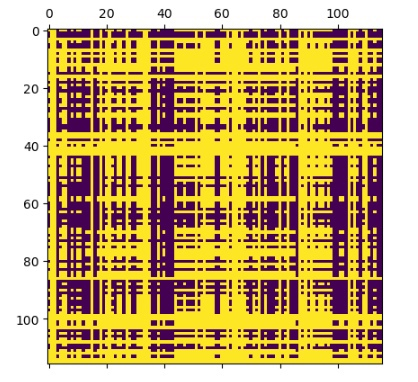
\includegraphics[width=0.49\textwidth]{Z_0.jpg}}
\subfigure[Estimated $\bPsi$]{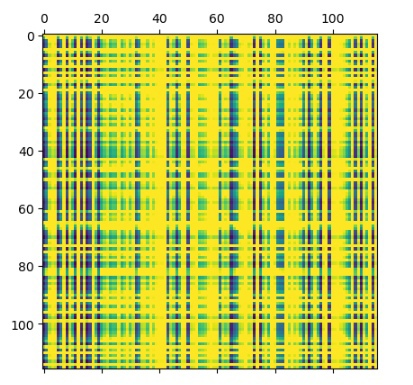
\includegraphics[width=0.49\textwidth]{Z_k.jpg}}
\caption{An example of the original matrix~$\bZ_0$ and the estimated matrix~$\bPsi$ for the problem of the Football Player List categorization}
\label{figMatrices}
\end{center}
\end{figure}
The fig.~\ref{figMatrices} shows the first stage of the proposed algorithm, an estimation of the matrix~$\bPsi$ using the matrices~$\bZ_0,\bZ_1,...,\bZ_n$.
The fig.~\ref{figMatrices} shows the original~$\bZ_0$ and the estimated~$\bPsi$ matrices for the Football Player List categorization problem. For this demonstration we construct a binary matrix~$\bZ_0$ shown at fig.~\ref{figMatrices}(a). The fig.~\ref{figMatrices}(b) shows the second stage of the algorithm for the Football Player List sample. The estimated matrix~$\bPsi$ is calculated without teacher. Every element of the matrix~$\bPsi(i,k)$ shows pairwise dominance of the objects~$\bx_k$~and~$\bx_i$.

\paragraph{Algorithms comparison}
The table~\ref{tab:AlgComparison} shows comparison of the proposed method with the method of decision oblique trees and with the isotonic regression. The loss function is Hamming distance between the class labels,
\[
s(y,\hat{y})=|y-\hat{y}|.
\]

\begin{table}[h]
\centering
\caption{Algorithm comparison on the Football Player dataset. The loss function is Hamming distance between class labels.}
\begin{tabular}{|c|c|c|}
  \hline
  Algorithm & Learn error & Test error \\
  \hline
  Partial Orders & 1.14 & 1.69 \\
  \hline
  Isotonic Regression & 0.98 & 1.28 \\
  \hline
  Oblique Decision Trees & 0.47 & 1.06 \\
  \hline
  Stochastic Partial Orders & 1.48 & 1.32 \\
  \hline
\end{tabular}
\label{tab:AlgComparison}
\end{table}

\section{Conclusion}
The proposed method of the ordinal classification problem uses partially ordered sets of expert estimations of features. We considered an alternative problem statement for the ordinal classification with monotonic constraints. Each partially ordered feature set corresponds to the partial order cone and to the matrix of the partial order graph. We find the solution of an ordinal classification problem as the projection to the cones superposition. The proposed method is compared with alternative approaches on the Football Player List dataset. The quality of classification was improved using the ideas considered in the present paper.

\bibliographystyle{unsrturl}
\bibliography{PartialOrdering}

\end{document}